\documentclass[a4paper,12pt,oneside]{article}

\usepackage{hyperref}
\usepackage[english,russian]{babel}
\usepackage[utf8]{inputenc}

%Возможность написания формул
\usepackage{amsmath}

%Препроцессинг графики
\usepackage{graphicx}
\newcommand{\anonsection}[1]{\section*{#1}\addcontentsline{toc}{section}{#1}}
\renewcommand{\theequation}{\arabic{section}.\arabic{equation}}

\title{Интеллектуальное сравнение текстов для поиска плагиата}
\author{Тямгин И.А. Белозуб В.А. Аметов О.З.}

\begin{document}
\maketitle
\anonsection{Аннотация}

Целью данной работы было исследование алгоритмов сравнения текстов для поиска плагиата в русскоязычном тексте и реализация нескольких из этих алгоритмов. Некоторые из рассмотренных алгоритмов были реализованы с небольшими изменениями и упрощениями.

\anonsection{Введение}
Большие объемы обрабатываемых данных делают задачу поиска похожих текстов алгоритмически сложной. При этом алгоритмы, успешно работающие для конкретной постановки задачи, бывают неприменимы или дают плохие результаты для других задач. Так, например, в юрислингвистике для определения авторства текста изучают его стилистические особенности, категоричность высказываний, использование оценочной лексики. Важно четко определить понятия плагиата и похожих текстов.

\section{Понятие плагиата}
\textit{Плагиат} — умышленное присвоение авторства чужого произведения искусства или достижения науки, технических решений или изобретений. Плагиат может быть нарушением авторско-правового законодательства и патентного законодательства и в качестве таковых может повлечь за собой юридическую ответственность. С другой стороны, плагиат возможен и в областях, на которые не распространяется действие каких-либо видов интеллектуальной собственности, например, в математике и других фундаментальных научных дисциплинах. [1]

В данной работе будем придерживаться именно этого определения, поскольку оно в той или иной форме приводится в большинстве статей, описывающих системы и алгоритмы определения плагиата.

~\\
Для разработки алгоритма важно определить два аспекта:
\begin{itemize}
\item Критерий определения похожести текстов (форма или содержание)
\item Определение оценки степени похожести и ее порогового значения, до которого тексты не считаются дубликатами.
\end{itemize}

Согласно классификации, приведенной в [3], случаи плагиата можно разделить на две основные группы: точное копирование и копирование с модификацией. Во втором случае текст может быть переформулирован или переведен на другой язык. Кроме того, может быть скопирован как целый текст, так и его часть. Алгоритмы, успешно обнаруживающие плагиат одного типа, могут давать очень слабые результаты для плагиата других типов.

\section{Постановка задачи}
Целью данной работы является исследование и разработка методов поиска плагиата в русскоязычных текстах. Для достижения данной цели были поставлены следующие задачи:
\begin{enumerate}
\item Исследовать существующие методы поиска плагиата.
\item Реализовать систему ставнения текстов, подтверждающую работоспособность данных методов.
\end{enumerate}

\section{Обзор существующих методов}
Существует ряд методов для нахождения плагиата в текстах. Наиболее часто процесс поиска осуществляется по следующему алгоритму:
\begin{enumerate}
\item Берут два текста, подозрительные на плагиат. 
\item Для этих двух документов анализируется степень сходства с проверяемым, если она достаточно высока – предполагается случай плагиата.
\item Пост-обработка. Полученные результаты проверяются, чаще всего вручную, для исключения ложных обнаружений (например, случаев, когда за плагиат принимается оформленная по всем правилам цитат).
\end{enumerate}

\subsection{Алгоритм шинглов}
Одним из наиболее часто используемых является метод «шинглов», предложенный в 1997 году. Он основан на представлении документа в виде всевозможных последовательностей фиксированной длины $k$, состоящих из соседних слов. Такие последовательности назвали «шинглами» (от англ. shingles). Два документа считаются похожими, если множества их шинглов существенно пересекаются. [2]

Данный подход можно разбить на такие основные этапы:
\begin{itemize}
\item канонизация текста
\item разбиение на шинглы
\item вычисление хэшей шинглов
\item сравнение, определение результата
\end{itemize}

\textbf{Канонизация текста}. Канонизация текста приводит оригинальный текст к единой нормальной форме. Текст очищается от предлогов, союзов, знаков препинания, HTML тегов, и прочего ненужного «мусора», который не должен участвовать в сравнении. В большинстве случаев также предлагается удалять из текста прилагательные, так как они не несут смысловой нагрузки.
Также на этапе канонизации текста можно приводить существительные к именительному падежу, единственному числу, либо оставлять от них только корни.

\textbf{Разбиение на шинглы}. \textit{Шинглы (англ — чешуйки)} — выделенные из статьи подпоследовательности слов. Необходимо из сравниваемых текстов выделить подпоследовательности слов, идущих друг за другом по $k$ штук (длина шингла). Выборка происходит внахлест, а не встык. Таким образом, разбивая текст на подпоследовательности, мы получим набор шинглов в количестве равному количеству слов минус длина шингла плюс один.

\textbf{Вычисление хэшей шинглов}. Принцип алгоритма шинглов заключается в сравнении случайной выборки контрольных сумм шинглов (подпоследовательностей) двух текстов между собой.
Проблема алгоритма заключается в количестве сравнений, ведь это напрямую отражается на производительности. Увеличение количества шинглов для сравнения характеризуется экспоненциальным ростом операций, что критически отразится на производительности.

\subsection{I-Match}

Рассмотрим другой сигнатурный подход, основанный уже не на синтаксических, а на лексических принципах. Для этого понадобиться понятия $TF$ и $IDF$ [4].

\textbf{TF} (term frequency — частота слова) — отношение числа вхождения некоторого слова к общему количеству слов документа. Таким образом, оценивается важность слова  в пределах отдельного документа.
\begin{equation} \mathrm{tf}(t,d) = \frac{n_i}{\sum_k n_k} \end{equation}
где $n_i$ есть число вхождений слова в документ, а в знаменателе — общее число слов в данном документе.

\textbf{IDF} (inverse document frequency — обратная частота документа) — инверсия частоты, с которой некоторое слово встречается в документах коллекции. Учёт IDF уменьшает вес широкоупотребительных слов. Для каждого уникального слова в пределах конкретной коллекции документов существует только одно значение IDF
\begin{equation} \mathrm{idf}(t, D) =  \log \frac{|D|}{|(d_{i}\supset t_{i})|} \end{equation}
где
\begin{itemize}
\item |D| — количество документов
\item $|(d_{i}\supset t_{i})|$ - — количество документов, в которых встречается $t_i$.
\end{itemize}

Выбор основания логарифма в формуле не имеет значения, поскольку изменение основания приводит к изменению веса каждого слова на постоянный множитель, что не влияет на соотношение весов.

Основная идея этого подхода, описанного в [3], состоит в вычислении дактилограммы I-Match для представления содержания документов. С этой целью сначала для исходной коллекции документов строится словарь $L$, который включает слова со средними значениями $IDF$. Слова с большими и маленькими значениями $IDF$ отбрасываются. Затем для каждого документа формируется множество $U$ различных слов, входящих в него, и определяется пересечение $U$ и словаря $L$. Если размер этого пересечения больше некоторого минимального порога (определяемого экспериментально), то список слов, входящих в пересечение упорядочивается, и для него вычисляется I-Match сигнатура (hash-функция).

Два документа считаются похожими, если у них совпадают I-Match сигнатуры. Алгоритм имеет высокую вычислительную эффективность, превосходящую показатели алгоритма шинглов. Другим преимуществом алгоритма (также, по сравнению с алгоритмом шинглов) является его высокая эффективность при сравнении небольших по размеру документов. Основной недостаток — неустойчивость к небольшим изменениям содержания документа.

\subsection{Слова с оптимальным весом}
Алгоритм реализует метод «оптимальной поисковой частоты», предложенный М. Масловым, и использующийся для поиска похожих документов в широком спектре приложений, от веб-поисковика до кластеризации новостей. Суть его заключается в следующем. Вместо классической метрики $TF*IDF$ предлагается ее модифицированный вариант. 

Вводится эвристическое понятие «оптимальной частоты» для слова равное \begin{equation} \ln \frac{10}{1000000} = 11.5 \end{equation} Т.е. «оптимальным» считается вхождение слова в 10 документов из
1000000. Если реальное значение $IDF$ меньше «оптимального», то оно немного (по закону параболы) повышается до
\begin{equation} IDF_{opt} = \sqrt{\frac{IDF}{11.5}} \end{equation}
а если больше, то существенно (как гипербола) снижается до
\begin{equation} IDF_{opt} = \frac{11.5}{IDF} \end{equation}
Таким образом по всей коллекции строится словарь, ставящий каждому слову в соответствие число документов, в которых оно встречается хотя бы один раз ($df$).
Далее строится частотный словарь документа и для каждого слова вычисляется его «вес» $ w_t $ по формуле:

\begin{equation} w_t = TF * IDF_{opt} \end{equation}
\begin{equation} TF = 0.5 + 0.5 * \frac{tf}{tf_{max}} \end{equation}
\begin{equation} IDF = -\log{\frac{tf}{N}} \end{equation}
\begin{equation} IDF_{opt} = \sqrt{IDF}{11.5} \end{equation}
если $IDF$ меньше чем 11.5, иначе
\begin{equation} IDF_{opt} = \frac{11.5}{IDF} \end{equation}

Затем выбираются и сцепляются в алфавитном порядке в строку слов с наибольшими значениями $ w_t $.

В качестве сигнатуры документа вычисляется контрольная сумма CRC32 полученной строки.

\subsection{Наиболее часто встречающиеся слова}
В качестве сигнатуры документа используется хэш-код строки, полученной сцеплением $k$ наиболее часто встречающихся в документа слов. Данный метод можно считать одним из случаев использования анализа ключевых слов текстов. Несмотря на свою простоту, при использовании нормализации и стоп-слов метод дает неплохие результаты.


\section{Практическая часть}
В качестве языка был выбран Python 2.7, являющийся кроссплатформенным языком, подходящим для работы со строками и регулярными выражениями, а также с протоколом http.

Из перечисленных выше методов выбраны два: алгоритм шинглов и I-Match.

Программа представляет собой веб-страницу, содержащую 2 текстовых поля ввода для сравниваемых документов, combobox для выбора длины шингла. Результат работы - вывод документов с выделенными фрагментами текста, которые присутствуют в обоих документах, которые показал алгоритм шинглов. Аналогично для I-Match.

Реализацию можно взять из репозитория https://github.com/tyamgin/IPI.git

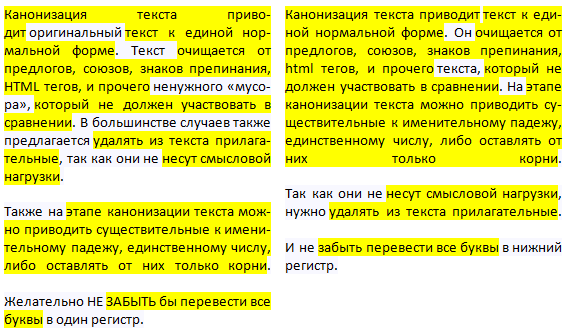
\includegraphics{a.png} 
\begin{center}
\textit{Рис 1. Результат работы алгоритма шинглов}
\end{center}

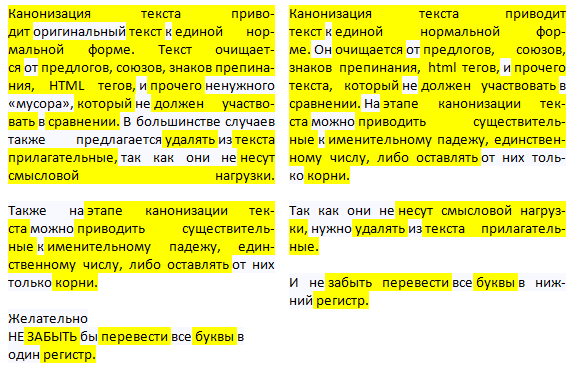
\includegraphics{b.png} 
\begin{center}
\textit{Рис 2. Результат работы алгоритма I-Match}
\end{center}

\newpage
\section{Заключение}
В рамках данной работы были получены следующие результаты:
\begin{enumerate}
\item Исследованы существующие методы поиска плагиата.
\item Построена система сравнения двух текстов, реализующая некоторые из рассмотренных подходов.
\end{enumerate}

\newpage	
\anonsection{Список использованных источников}
\begin{enumerate}
\item Определение плагиата. https://ru.wikipedia.org/wiki/Плагиат
\item Алгоритм шинглов. https://ru.wikipedia.org/wiki/Алгоритм\_шинглов
\item Зеленков Ю.Г., Сегалович И.В. Cравнительный анализ методов определения нечетких дубликатов для WEB-документов // Труды 9-ой Всероссийской научной конференции «Электронные библиотеки: перспективные методы и технологии, электронные коллекции» RCDL’2007: Сб. работ участников конкурса, том 1. Переславль-Залесский, Россия: «Университет города Переславля», 2007. С. 166-174
\item TF-IDF. https://ru.wikipedia.org/wiki/TF-IDF
\end{enumerate}

\end{document}